\chapter{Hardware}
\label{chap:hardware}

This chapter presents the general architectures of a CPU and a GPU.
Furthermore, we present Amdahl's Law and Gustafson-Barsis Law, which discuss two different aspects of parallel execution compared to sequential execution.
We end the chapter by discussing why it is not a good idea to go all in with the GPU and no longer use a CPU.

First, we present \cref{tab:hardware connections transfer rates} which summarises the transfer rates of different connections of the different types of hardware.
We add \cref{fig:cpu gpu communication} to illustrate the connections these have.\todo{add table and figure}

\section{CPU Architecture}
\label{sec:cpu}
The Central Processing Unit (CPU) is the processing unit in a modern day computer.
The CPU handles processing and control of data in the computer's memory space.
The CPU is usually made of a small amount of complex cores, referred to as Multiple Instruction, Multiple Data (MIMD) Arithmetic Logic Units (ALU) that are optimized for reducing the latency of a given task.

The bottleneck of computation is often placed at the memory's ability to transfer data to/from the CPU, also known as Input/Output (I/O).
To increase the I/O the CPU has a built-in memory architecture with high speed, but low storage capabilities.
The optimized memory architecture allows the CPU the store, ``cache'', memory for later reuse and thus reduce the memory bottleneck.~\cite{bryant2003computer}

\section{General GPU Architecture}
\label{sec:gpu}

The Graphical Processing Unit (GPU) is a device which is attached to a host machine.
This means that the GPU is an attached piece of hardware, which then is a work horse that works together with the CPU to perform computations.
We present \cref{fig:sm example} as a reference for this section.

\begin{figure}[htb]
  \centering
  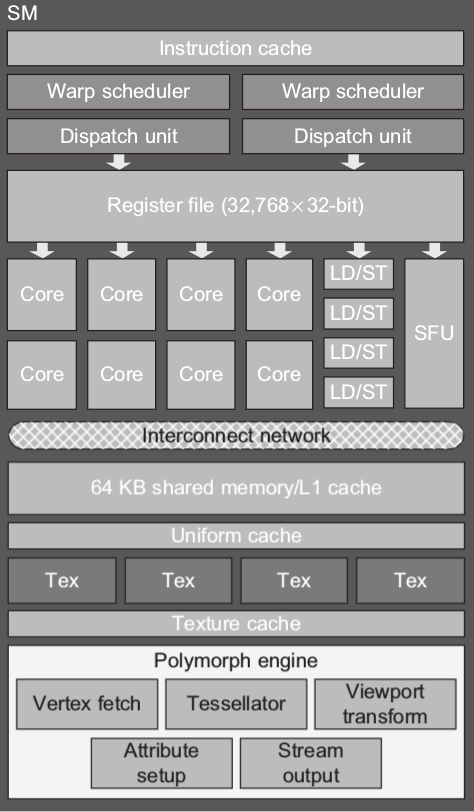
\includegraphics[width=.5\textwidth]{graphics/images/cropped-cuda-sm.png}
  \caption{Example of a Streaming Multiprocessor for reference~\cite{farber2011cuda}}
  \label{fig:sm example}
\end{figure}

A GPU's basic building block is the streaming multiprocessor (SM), which is independently responsible for its own resources, cores, and memory.
By making each SM independent memory access and computation are performed faster, because there is not global memory or special units that are shared among all the hardware.
Each SM has Single Instruction Multiple Data (SIMD) Arithmetic Logic Units (ALU), which are commonly referred to as the cores.
These cores will all run the same instruction, but may use different data.

The work given to the GPU is distributed to the SMs by the Giga-Thread global scheduler, which knows when the SMs are busy.
CUDA-enabled devices are categorised by their compute capability which describes the amount of threads each block can have.
Threads actually perform computations.
They are organised into blocks and grids.
These are described further in \cref{chap:software}.

The SMs receive instructions in a cache and warp schedulers distribute the work to the cores, so the instructions can be executed.
Each thread has access to its own registers, which is called its local memory.
Each SM has shared memory for high-speed data sharing between threads in a block.
The GPU as a whole has memory called global memory, which is accessible by all the GPU's SMs.

Furthermore, an SM has load/store (LD/ST) units and Special Function Units (SFU).
LD/STs calculate source and destination addresses and loads/store data as needed.
SFUs execute special functions, e.g. sin, sqrt, etc.
Each SFU executes one instruction per thread per clock.
SFUs can perform an operation while it is communicating with another thread.
Compared to the SIMD cores, the SFUs are designed specifically to perform their designated functions, and the SIMD cores are general purpose cores.

% good warp answers:  http://stackoverflow.com/questions/11816786/why-bother-to-know-about-cuda-warps
%                     http://stackoverflow.com/questions/10460742/how-do-cuda-blocks-warps-threads-map-onto-cuda-cores
A warp is a block of 32 SIMD threads, and they are the basic unit for scheduling work in the SMs.
To maximize the utilisation of the GPU the developer must make sure that these warp sizes are considered when executing code.
If one does not consider the warp size and randomly schedules tasks, then the programs might have many idle threads that do nothing.
If this is the case, then the GPU is not utilised to its optimal capacity~\cite{fermi2009nvidia}.

\subsection{Hardware Specific Numbers}
\label{sec:hardware specific numbers}

Throughout this report, we will be using the Tesla K40 GPU~\cite{teslak402013nvidia}.
For future reference \cref{tab:tesla k40 specs} presents the specifications for our GPU device.
In \cref{ap:tesla k40 specifications} we walk through how we found the specifications for our device.
\todo{is L1 cache used for shared memory?}

\begin{table}[htb]
  \centering
  \begin{tabular}{l r}
    \toprule
    item                        & limit \\
    \midrule
    warp size                   & \SI{32}{} \\
    max threads / block         & \SI{1024}{} \\
    total cores                 & \SI{2880}{} \\
    registers / block           & \SI{65536}{} \\
    constant memory             & \SI{65536}{B} \\
    L1 cache / block            & \SI{49152}{B}  \\
    L2 cache / core             & \SI{1572864}{B}  \\
    global memory               & \SI{12079136768}{B} \\
    \bottomrule
  \end{tabular}
  \caption{Tesla K40 GPU's specifications}
  \label{tab:tesla k40 specs}
\end{table}

Furthermore, the maximum dimension of grids and blocks are presented in \cref{tab:tesla k40 grid and block}.

\begin{table}[htb]
  \centering
  \begin{tabular}{r r r r}
    \toprule
    item & x & y & z \\
    \midrule
    block size & \SI{1024}{} & \SI{1024}{} & \SI{64}{} \\
    grid size  & \SI{2147483647}{} & \SI{65535}{} & \SI{65535}{} \\
    \bottomrule
  \end{tabular}
  \caption{Tesla K40 GPU's block and grid sizes}
  \label{tab:tesla k40 grid and block}
\end{table}

\section{Parallel Performance}
\label{sec:parallel performance}

This section presents two models that aims to assess theoretical performance speed up with parallel computing.
Both models ignores overhead costs, memory transfers and synchronization.

The first is model i known as Amdahl's Law, which attempts to describes how much faster a program can execute while holding the workload constant.
The second model is known as Gustafson-Barsis Law, which describes how much more work can be performed holding the running time constant.

\subsection{Amdahl's Law}
\label{sec:amdahls law}

Amdahl's Law approximates the potential speed up of a serial program.
The equation is presented in \cref{eq:amdahls law}, where $P$ is the portion of the serial code that can be parallelized, $(1-P)$ is the portion that cannot be parallelized and $n$ is the amount of processors available.
Thus, $S(n)$ is the theoretical speed up achievable while holding the workload constant.

\begin{equation}
  \label{eq:amdahls law}
  S(n) = \frac{1}{(1-P) + P/n}
\end{equation}

Amdahl's Law only applies if the amount of work performed in the parallel version is not significantly different than the serial code's amount of work.
An illustration of the potential speed up is presented in \cref{fig:amdahls law} with $n=1024$.
The model thus theorize that given a fully parallizable problem, the problem should be executed $n$ times faster~\cite{farber2011cuda}.

\begin{figure}[htb]
  \centering
  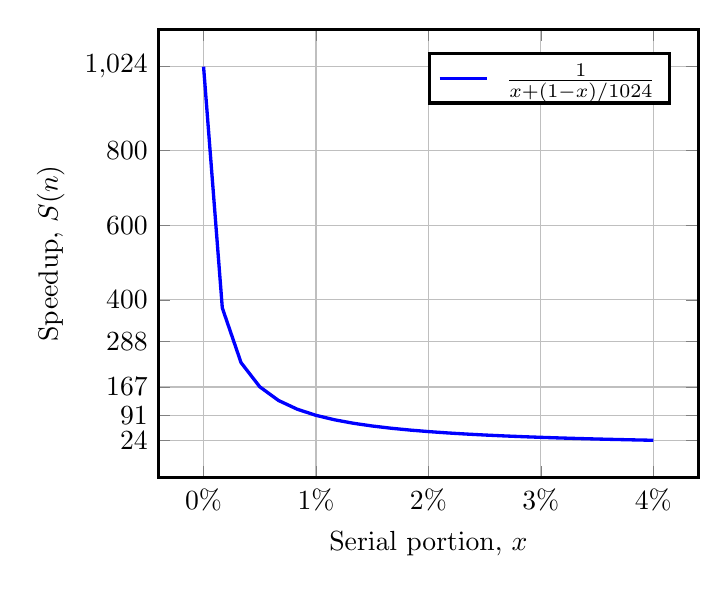
\begin{tikzpicture}
  \begin{axis}[
    ymajorgrids,
    xmajorgrids,
    ylabel={Speedup, $S(n)$},
    ytick={24,91,167,288,400,600,800,1024},
    xlabel={Serial portion, $x$},
    scaled x ticks = false, % do not add axis-multiplier
    xticklabel={% print percent
      \pgfmathparse{\tick*100}%
      \pgfmathprintnumber{\pgfmathresult}%
      \%%
    },
    legend style={
      at={(0.95,0.95)},
      anchor=north east,
      column sep=1ex
     },
     no markers,
     very thick
  ]

  \addplot+[domain=0.00:0.04] {1/(x+((1-x)/1024))};
  \addlegendentry{$\frac{1}{x + (1-x) / 1024}$};
  \end{axis}
\end{tikzpicture}

  \caption{Speed up by Amdahl's Law, where $x=(1-P)$, $(1-x)=P$, and $n=1024$}
  \label{fig:amdahls law}
\end{figure}

An important property of Amdahls is the decline of the curve as the solution moves from 0\% to 1\%.
With parallel portion $P=0.99$ the speed up is approximately $91\times$, and $1024\times$ when $P=1.00$ and everything can be made parallel.
According to Amdahl's Law, with just a tiny portion of the code that cannot become parallel, a high speed up is not likely to be achieved.

\subsection{Gustafson-Barsis Law}
\label{sec:gustafson-barsis law}

Gustafson and Barsis Law approximates how much more throughput can be achieved by increasing processor count in a defined amount of time.
This type of formulation is often interesting when computing problems that are open ended such as computing pi -- given more computational power, the processors can compute more digits of pi in the same time~\cite{amdahlorgustafson2011}.

\begin{equation}
  \label{eq:gustafson-barsis law}
  W(n) = n + (1-n) \times (1-P)
\end{equation}
Where $P$ is the amount of the program that can be parallelized and $W(n)$ is the theoretical increase in throughput over a defined period of time.

\todo{rewrite below - Alex}
 achievable,defines the amount of 
So, the goal is to run a program in the same amount of time but with more work.
This approximation is present in \cref{eq:gustafson-barsis law}.
Thus, $W(n)$ gives the amount of work that can be further performed~\cite{gustafson1988reevaluating}.


% cpu vs. gpu: http://superuser.com/questions/308771/why-are-we-still-using-cpus-instead-of-gpus
\section{Do we ditch the CPU, and keep the GPGPU?}
\label{sec:cpu vs gpu}

It is true that a GPGPU has many more cores than a CPU, but the cores are significantly slower than the ones in a CPU.
The GPGPU neither have features for more general computer such as interrupts and virtual memory (used in modern day operating systems).
As a result, the two processing units are developed with two different goals and thus have different characteristics.

As every type of problem might not have a parallel solution, and writing parallel code is a lot trickier than serial code, the CPU is still very much needed.
The role of the GPGPU has thus evolved to be an "accelerator" to the CPU, a specialized computing unit to accelerate parallelisable tasks.
At runtime the CPU will thus initialize the GPGPU and send it data to process when faced with such parallelisable tasks, the relationship is called a host (CPU) to device (GPGPU) relationship.

